%%%%%%%%%%%%%%%%%%%%%%%%%%%%%%%%%%%%%%%%%%%%%%%%%%%%%%%%%%%%%%%%%%%%%%
% Lớp 11 | Hàm số lượng giác và phương trình lượng giác | Giá trị lượng giác của một góc lượng giác
% Dạng 1D1?2-1: Câu hỏi lý thuyết
% Số câu: 39  (sinh tự động bởi tach_cau.py; từ nay thầy sửa trực tiếp file này)
%%%%%%%%%%%%%%%%%%%%%%%%%%%%%%%%%%%%%%%%%%%%%%%%%%%%%%%%%%%%%%%%%%%%%%

%%%%%%%%%%%%%%%% TRẮC NGHIỆM 4 PHƯƠNG ÁN %%%%%%%%%%%%%%%%

% nguồn: Ok_Toan11_TracNghiem_Lan2
\begin{ex}%[1D1N2-1]%[ma:96c724d9]
	Cho $\dfrac{\pi}{2} < \alpha < \pi$. Giá trị lượng giác nào sau đây  luôn dương?
	\choice 
		{$\sin  \left(\pi+\alpha \right)$}
		{\True $\cos  \left(\dfrac{\pi}{2}-\alpha \right)$}
		{$\cos  \left(-\alpha \right)$}
		{$\tan \left(\pi+\alpha \right)$} 
	\loigiai{ 
		Do $\dfrac{\pi}{2} < \alpha < \pi $ nên $\heva{&{\sin \alpha >  0} \\
		 &{\cos \alpha < 0} \\
		 &{\tan \alpha < 0.}
		 }$
	} 
\end{ex}

% nguồn: Ok_TracNghiemLop11_Lan1
\begin{ex}%[1D1N2-1]%[ma:d5d6422e]
	Trên đường tròn lượng giác gốc $A(1;0)$, cho cung $\overset{\curvearrowright}{AM}$ có $\text{sđ}\,\overset{\curvearrowright}{AM}=\dfrac{8\pi}{3}$.  Tìm tọa độ của điểm $M$.
	 \choice
		{$\left( \dfrac{\sqrt{3}}{2}; -\dfrac{1}{2} \right)$} 
		{$\left( \dfrac{\sqrt{3}}{2};  \dfrac{1}{2} \right)$}
		{\True $\left(  -\dfrac{1}{2}; \dfrac{\sqrt{3}}{2} \right)$}
		 {$\left( \dfrac{1}{2}; -\dfrac{\sqrt{3}}{2} \right)$}
	 \loigiai{
		Ta có $\cos  \dfrac{8\pi}{3}=-\dfrac{1}{2}$ và $\sin \dfrac{8\pi}{3}=\dfrac{\sqrt{3}}{2}$ nên $M\left( -\dfrac{1}{2}; \dfrac{\sqrt{3}}{2} \right)$.
	} 
\end{ex}

% nguồn: Ok_TracNghiemLop11_Lan1
\begin{ex}%[1D1N2-1]%[ma:db10882a]
	Trong các hệ thức  sau đây, hệ thức nào đúng?
	 \choice
		 {\True $\sin^2x+\cos^2x=1$}
		{$\sin{x^2}+\cos{x^2}=1$} 
		 {$\sin 2x+\cos 2x=1$}
		 {$\sin^2x+\cos{x^2}=1$}
	 \loigiai{
		 $\sin^2x+\cos^2x=1$.
	 }
\end{ex}

% nguồn: Ok_TracNghiemLop11_Lan1
\begin{ex}%[1D1N2-1]%[ma:43374932]
	\immini 
	{Cho góc lượng giác có số đo bằng $\dfrac{-3\pi}{4}$. Điểm nào sau đây  là điểm biểu diễn góc lượng giác đã cho trên đường tròn lượng giác?
	\choice 
		{Điểm  $A$}
		{Điểm  $B$}
		{\True Điểm  $C$}
		 {Điêm $D$}}
		{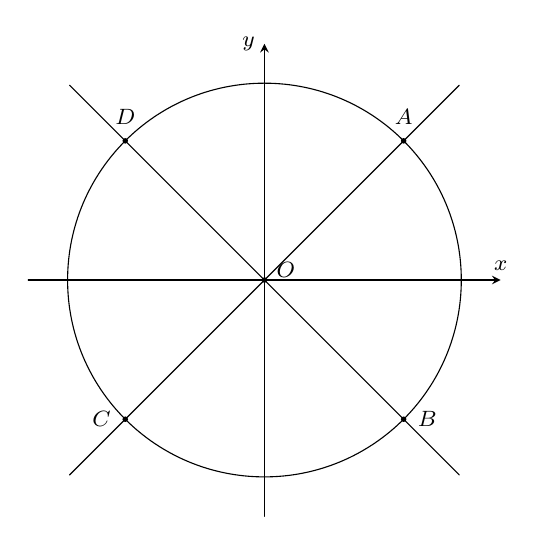
\begin{tikzpicture}[line join=round,line cap=round,>=stealth,font=\footnotesize,scale=1]
		\def\r{2.5} 
		\draw[-stealth]  (-3,0)--(3,0) node[above]{$x$};
		 \draw[-stealth] (0,-3)--(0,3) node[left]{$y$};
		\draw (45:\r+1)--(225:\r+1)  node[above]{};
		\draw (135:\r+1)--(315:\r+1)  node[left]{};
		 \path
			(0,0) coordinate (O) 
			 (45:\r) coordinate (A)
			(135:\r)  coordinate (D)
			 (225:\r) coordinate (C)
			 (315:\r) coordinate (B);
		\draw (O) circle (\r); 
		\foreach \p/\r  in {O/25,A/90,B/0,D/90,C/180}
		\fill (\p)  circle (1pt) node[shift={(\r:3mm)}]{$\p$};
	\end{tikzpicture}
		 }
	 \loigiai{
		Điểm $C$ nằm ở vị  trí $-135^\circ=-\dfrac{3\pi}{4}$.
	} 
\end{ex}

% nguồn: Ok_TracNghiemLop11_Lan1
\begin{ex}%[1D1N2-1]%[ma:43d99e9d]
	Trong các liên hệ giữa các giá trị  lượng giác sau, liên hệ nào là \textbf{sai}?
	 \choice
		{\True $\cos\left(\dfrac{\pi}{2}-\alpha\right)=\cos(\alpha)$} 
		{$\cos(-\alpha)=\cos(\alpha)$} 
		 {$\cos(\pi-\alpha)=-\cos(\alpha)$}
		{$\cos(\pi+\alpha)=-\cos(\alpha)$} 
	\loigiai{ 
		Vì $\cos\left(\dfrac{\pi}{2}-\alpha\right)=\sin(\alpha)$. 
	} 
\end{ex}

% nguồn: Ok_TracNghiemLop11_Lan1
\begin{ex}%[1D1N2-1]%[ma:5bc3c4aa]
	Tập nghiệm $S$ của phương  trình $3\tan x-\sqrt{3}=0$ là
	 \choice
		{$S=\left\{\dfrac{\pi}{6}+\dfrac{k2\pi}{3}\mid k\in  \mathbb{Z}\right\}$}
		{\True $S=\left\{\dfrac{\pi}{6}+k\pi\mid k\in \mathbb{Z}\right\}$} 
		{$S=\left\{\dfrac{\pi}{6}+k2\pi\mid  k\in \mathbb{Z}\right\}$}
		{$S=\left\{\dfrac{\pi}{6}+\dfrac{k\pi}{3}\mid k\in  \mathbb{Z}\right\}$}
	 \loigiai{
		Ta có $3\tan x-\sqrt{3}=0\Leftrightarrow \tan  x=\dfrac{\sqrt{3}}{3}\Leftrightarrow x=\dfrac{\pi}{6}+k\pi$, $k\in \mathbb{Z}$. \\
	Vậy tập nghiệm của phương trình là $S=\left\{\dfrac{\pi}{6}+k\pi\mid  k\in \mathbb{Z}\right\}$.}
\end{ex}

% nguồn: Ok_TracNghiemLop11_Lan1
\begin{ex}%[1D1H2-1]%[ma:a7547405]
	Phương trình $ \tan x=\tan\left(\dfrac{-\pi}{3}\right)$ có tất cả các  nghiệm là
	\choice 
		{\True  $x=\dfrac{-\pi}{3}+k\pi$, $(k\in\mathbb{Z})$}
		 {$x=\pm \dfrac{\pi}{3}+k\pi$, $(k\in\mathbb{Z})$}
		 {$x=\dfrac{-\pi}{3}+k2\pi$, $(k\in\mathbb{Z})$}
		{$x=\dfrac{\pi}{3}+k2\pi$, $(k\in\mathbb{Z})$} 
	 \loigiai{
		$\tan  x=\tan\left(\dfrac{-\pi}{3}\right) \Leftrightarrow x=\dfrac{-\pi}{3}+k\pi$, $(k\in\mathbb{Z})$.
	 }
\end{ex}

% nguồn: Ok_TracNghiemLop11_Lan1
\begin{ex}%[1D1Y2-1]%[ma:da67d729]
	Tìm tập nghiệm của  phương trình $2 \cos \left( 3x+\dfrac{\pi}{4} \right) +\sqrt{3}=0$.
	 \choice
		{$\left\lbrace \dfrac{7\pi}{36} + k 2\pi , -\dfrac{13\pi}{36}+k 2 \pi | k \in  \mathbb{Z} \right\rbrace $}
		{\True $\left\lbrace \dfrac{7\pi}{36} + k\dfrac{2\pi}{3}, - \dfrac{13\pi}{36}+k\dfrac{2\pi}{3} | k \in \mathbb{Z} \right\rbrace $} 
		{$\left\lbrace \pm \dfrac{5\pi}{6} + k 2\pi| k \in \mathbb{Z}  \right\rbrace $}
		{$\left\lbrace - \dfrac{7\pi}{36} + k\dfrac{2\pi}{3}, \dfrac{13\pi}{36}+k\dfrac{2\pi}{3}  | k \in \mathbb{Z} \right\rbrace $}
	 \loigiai{
		Phương trình đã cho tương đương với 
		\begin{eqnarray*}
			\cos \left( 3x +\dfrac{\pi}{4}\right) = -\dfrac{\sqrt{3}}{2} &\Leftrightarrow& 
			\hoac{&3x + \dfrac{\pi}{4} = \dfrac{5\pi}{6} + k2\pi, k \in \mathbb{Z}  \\ & 3x+ \dfrac{\pi}{4} = -\dfrac{5\pi}{6} + k2\pi , k\in \mathbb{Z}} \\
			&\Leftrightarrow& \hoac{& x= \dfrac{7\pi}{36} +  \dfrac{k2\pi}{3}, k \in \mathbb{Z} \\ & x= -\dfrac{13\pi}{36} + \dfrac{k2\pi}{3}, k \in \mathbb{Z}.}
		\end{eqnarray*}
	} 
\end{ex}

% nguồn: Ok_TracNghiemLop11_Lan1
\begin{ex}%[1D1Y2-1]%[ma:318ad877]
	Trong các  phương trình sau, phương trình nào vô nghiệm?
	\choice 
		{$\sin x-\cos  x=1$}
		{$\cot x=2018$} 
		 {\True $\sin x=2$}
		{$\sin x=-\dfrac{3}{4}$} 
	 \loigiai{
		Vì $\sin x\in[-1;1]$  nên phương trình $\sin x=2$ vô nghiệm.
	 }
\end{ex}

% nguồn: Ok_TracNghiemLop11_Lan1
\begin{ex}%[1D1B2-1]%[ma:7879be5f]
	Nghiệm của phương trình $ 2\cos \dfrac{x}{2}+\sqrt{3}=0$ là 
	 \choice
		{$  x=\pm\dfrac{5\pi}{6}+k2\pi ,k\in\mathbb{Z} $}
		{\True  $ x=\pm\dfrac{5\pi}{3}+k4\pi ,k\in\mathbb{Z}$}
		 {$x=\pm\dfrac{5\pi}{3}+k2\pi ,k\in\mathbb{Z} $}
		{$x=\pm\dfrac{5\pi}{6}+k4\pi ,k\in\mathbb{Z} $} 
	 \loigiai{
		Phương trình tương đương với $$\cos  \dfrac{x}{2}=-\dfrac{\sqrt{3}}{2}\Leftrightarrow\dfrac{x}{2}=\pm \dfrac{5\pi}{6}+k2\pi\Leftrightarrow x=\pm\dfrac{5\pi}{3}+k4\pi,\,k\in\mathbb{Z}.$$
	 }
\end{ex}

% nguồn: Ok_TracNghiemLop11_Lan1
\begin{ex}%[1D1B2-1]%[ma:5fa200b3]
	Phương  trình: $\sin x =\cos 5x$ có các nghiệm là
	 \choice
		{$x=\dfrac{\pi}{4}+k2\pi$ và $x=\dfrac{-\pi}{4}+k2\pi  , (k \in \mathbb{Z})$}
		{$x=\dfrac{-\pi}{12}+k\dfrac{\pi}{3}$ và  $x=\dfrac{\pi}{8}+k\dfrac{\pi}{2} , (k \in \mathbb{Z})$}
		{$x=\dfrac{\pi}{4}+k\pi$  và $x=\dfrac{-\pi}{4}+k\pi , (k \in \mathbb{Z})$}
		 {\True $x=\dfrac{\pi}{12}+k\dfrac{\pi}{3}$ và $x=\dfrac{-\pi}{8}+k\dfrac{\pi}{2} , (k \in \mathbb{Z})$}
	\loigiai{ 
		Ta có 
		\begin{eqnarray*}
			 & & \sin x =\cos 5x \\
			&\Leftrightarrow & \sin x = \sin \left(\dfrac{\pi}{2}-5x\right)\\ 
			&\Leftrightarrow & \hoac{& x=\dfrac{\pi}{2}-5x+k2\pi\\  &x = \dfrac{\pi}{2} + 5x + k2\pi}\\
			&\Leftrightarrow & \hoac{&  x=\dfrac{\pi}{12}+k\dfrac{\pi}{3}\\ &x=\dfrac{-\pi}{8}+k\dfrac{\pi}{2}}(k \in \mathbb{Z}).
		\end{eqnarray*}
	} 
\end{ex}

% nguồn: Ok_TracNghiemLop11_Lan1
\begin{ex}%[1D1Y2-1]%[ma:934609de]
	Nghiệm của phương trình $\cos \left(x+\dfrac{\pi }{3}\right)=0$ là 
	\choice 
		{ $ x=-\dfrac{\pi  }{3}+k\pi; ~k\in \mathbb{Z}$}
		{\True $  x=\dfrac{\pi }{6}+k2\pi; ~k\in \mathbb{Z}$}
		{ $  x=-\dfrac{5\pi }{6}+k2\pi; ~k\in \mathbb{Z}$}
		{ $ x=\dfrac{25\pi }{6}+k\pi; ~k\in \mathbb{Z}$} 
	 \loigiai{
		 Ta có $\cos \left(x+\dfrac{\pi }{3}\right)=0\Leftrightarrow x+\dfrac{\pi }{3}=\dfrac{\pi }{2}+k2\pi \Leftrightarrow x=\dfrac{\pi }{6}+k2\pi $, $ k\in \mathbb{Z}$.
	} 
\end{ex}

% nguồn: Ok_TracNghiemLop11_Lan1
\begin{ex}%[1D1Y2-1]%[ma:15754c25]
	Phương trình $ \sin \left(x-\dfrac{\pi}{3}\right)=1 $  có nghiệm là
	\choice 
		{$x=\dfrac{5\pi}{6}+k\pi, k\in \mathbb{Z} $} 
		 {$x=\dfrac{\pi}{3}+k2\pi, k\in \mathbb{Z} $}
		{\True $x=\dfrac{5\pi}{6}+k2\pi, k\in  \mathbb{Z} $}
		 {$x=\dfrac{\pi}{3}+k\pi, k\in \mathbb{Z} $}
	 \loigiai{
		Ta có: $\sin \left(x-\dfrac{\pi}{3}\right)=1\Leftrightarrow x-\dfrac{\pi}{3}=\dfrac{\pi}{2}+k2\pi, k\in \mathbb{Z}\Leftrightarrow x=\dfrac{5\pi}{6}+k2\pi, k \in  \mathbb{Z} $.
	 }
\end{ex}

% nguồn: Ok_TracNghiemLop11_Lan1
\begin{ex}%[1D1Y2-1]%[ma:17a8e0bd]
	Giải  phương trình $ 2\cos x-1=0 $.
	\choice 
		{$x=\pm  \dfrac{\pi}{3}+2\pi, k\in \mathbb{Z} $}
		{\True $x=\pm \dfrac{\pi}{3}+k2\pi, k\in \mathbb{Z} $} 
		{$x=\pm  \dfrac{\pi}{6}+k2\pi, k\in \mathbb{Z} $}
		{$x=  \dfrac{\pi}{3}+k2\pi, k\in \mathbb{Z} $}
	 \loigiai{
		Ta có $ 2\cos x-1=0  \Leftrightarrow \cos x=\dfrac{1}{2}\Leftrightarrow x=\pm \dfrac{\pi}{3}+k2\pi, k\in \mathbb{Z}$.
	 }
\end{ex}

% nguồn: Ok_TracNghiemLop11_Lan1
\begin{ex}%[1D1B2-1]%[ma:cb742e95]
	Nghiệm lớn nhất của phương trình $2\cos 2x-1=0$ trong  đoạn $\left[0;\pi \right]$ là
	 \choice
		{$x=\dfrac{2\pi}{3}$} 
		{$x=\dfrac{11\pi}{12}$} 
		{\True $x=\dfrac{5\pi}{6}$} 
		{$x=\pi $} 
	 \loigiai{
		Ta có $2\cos 2x-1=0 \Leftrightarrow \cos 2x=\dfrac{1}{2}=\cos \dfrac{\pi}{3}  \Leftrightarrow \left[
		\begin{aligned}
			&x=\dfrac{\pi}{6}+k\pi  \\
			 &x=-\dfrac{\pi}{6}+k\pi
		\end{aligned}\right. (k\in \mathbb{Z})$. \\
	Vì  $x\in \left[0;\pi \right] $ nên $ x\in \left\{\dfrac{\pi}{6};\dfrac{5\pi}{6}\right\}$.}
\end{ex}

% nguồn: Ok_TracNghiemLop11_Lan1
\begin{ex}%[1D1B2-1]%[ma:c116e432]
	Cho phương trình $\sin{x}-\sin{2x}+\sin{3x}=0$. Nghiệm  của phương trình là
	\choice 
		{$x=\dfrac{\pi}{2}+k2\pi; x=k\pi, k\in \mathbb{Z}$} 
		 {$x=k\dfrac{\pi}{2}+k\pi, k\in \mathbb{Z}$}
		{\True $x=\pm \dfrac{\pi}{3}+k2\pi;  x=k\dfrac{\pi}{2}, k\in \mathbb{Z}$}
		{$x=\pm  \dfrac{\pi}{6}+k\pi, k\in \mathbb{Z}$}
	\loigiai{ 
		Phương trình $\sin{x}-\sin{2x}+\sin{3x}=0$ tương đương  với
		\begin{eqnarray*}
			2\sin{2x}\cos{x}-\sin{2x}=0 &\Leftrightarrow&  \sin{2x}(2\cos{x}-1)=0\\
			&\Leftrightarrow& \hoac{&\sin{2x}=0\\&\cos{x}=\dfrac{1}{2}} \;\Leftrightarrow\; \hoac{&x=\dfrac{k\pi}{2}\\&x=\pm\dfrac{\pi}{3}+k2\pi}  \,(k\in \mathbb{Z}).
		\end{eqnarray*}
	} 
\end{ex}

% nguồn: Ok_TracNghiemLop11_Lan1
\begin{ex}%[1D1Y2-1]%[ma:44439d63]
	 Nghiệm của phương trình $\sin x=\dfrac{1}{2}$ là
	 \choice
		{$x=\pm \dfrac{\pi}{6}+k2\pi$} 
		{\True $x=\dfrac{\pi}{6}+k2\pi$  và $x=\dfrac{5\pi}{6}+k2\pi$}
		{$x=\dfrac{\pi}{6}+k\pi$ và $x=\dfrac{5\pi}{6}+k\pi$} 
		{$x=-\dfrac{\pi}{6}+k2\pi$ và $x=-\dfrac{5\pi}{6}+k2\pi$} 
	\loigiai{ 
		 $$\sin x=\dfrac{1}{2}
		\Leftrightarrow \sin x= \sin \dfrac{\pi}{6} 
		\Leftrightarrow  \hoac{&x=\dfrac{\pi}{6}+k2\pi\\&x=\dfrac{5\pi}{6}+k2\pi.}$$
	} 
\end{ex}

% nguồn: Ok_TracNghiemLop11_Lan1
\begin{ex}%[1D1Y2-1]%[ma:b0967768]
	Phương trình $\cos 2x=m$ vô nghiệm khi $m$  thỏa
	\choice 
		 {\True $\left[
		\begin{aligned}
			&m<-1\\ 
			&m>1\\ 
	\end{aligned}\right. $}
	{$m>1$} 
	{$-1 \leqslant  m \leqslant 1$}
	 {$m<-1$}
	\loigiai{ 
		Ta có:  $\left|\cos x\right| \leqslant 1,\,\forall x \in \mathbb{R}$.\\
		Do đó, phương trình $\cos 2x=m$ vô nghiệm $ \Leftrightarrow |m|>1 \Leftrightarrow \left[ 
		\begin{aligned}
			&m<-1\\ 
			&m>1\\ 
	\end{aligned}\right. $.}
\end{ex}

% nguồn: Ok_TracNghiemLop11_Lan1
\begin{ex}%[1D1Y2-1]%[ma:31089cc6]
	Tập nghiệm  của phương trình $\sin 2x=\sin x$ là
	 \choice
		{$S=\left\{k2\pi;\pi+k2\pi\left|k\in  \mathbb{Z}\right. \right\}$}
		{\True $S=\left\{k2\pi;\dfrac{\pi}{3}+\dfrac{k2\pi}{3}\left|k\in \mathbb{Z}\right. \right\}$} 
		{$S=\left\{k2\pi;\dfrac{\pi}{3}+k2\pi\left|k\in \mathbb{Z}\right. \right\}$} 
		{$S=\left\{k2\pi;-\dfrac{\pi}{3}+k2\pi\left|k\in \mathbb{Z}\right.  \right\}$}
	 \loigiai{
		Ta có $\sin 2x=\sin  x \Leftrightarrow \left[
		\begin{aligned}
			 &2x=x+k2\pi \\
			&2x=\pi-x+k2\pi 
		\end{aligned}\right. \Leftrightarrow \left[
		\begin{aligned}
			&x=k2\pi \\ 
			 &x=\dfrac{\pi}{3}+\dfrac{k2\pi}{3}
	\end{aligned}\right. \left(k\in \mathbb{Z}\right)$.}
\end{ex}

% nguồn: Ok_TracNghiemLop11_Lan1
\begin{ex}%[1D1Y2-1]%[ma:89c77e36]
	Khẳng định nào  sau đây là đúng
	\choice 
		{$\cos x =0 \Leftrightarrow x =\dfrac{\pi}{2} +k2\pi; k \in  \mathbb{Z}$}
		{\True $\cos x =-1  \Leftrightarrow x =\pi +k2 \pi; k \in \mathbb{Z}$}
		{$\sin x =0 \Leftrightarrow x = k2\pi;  k \in \mathbb{Z}$}
		 {$\tan x =0 \Leftrightarrow x = k 2\pi; k \in \mathbb{Z}$}
	\loigiai{ 
		Ta có $\cos x =-1 \Leftrightarrow  x =\pi +k2 \pi; k \in \mathbb{Z}$.
	 }
\end{ex}

% nguồn: Ok_TracNghiemLop11_Lan1
\begin{ex}%[1D1B2-1]%[ma:728e01ef]
	Phương trình $\sin^2  x+\cos 2x=-\cos^2 x$ có nghiệm là
	 \choice
		{$x=k2\pi, (k\in  \mathbb{Z})$}
		 {$x=\pi+k2\pi, (k\in \mathbb{Z})$}
		 {\True $x=\dfrac{\pi}{2}+k\pi, (k\in \mathbb{Z})$}
		 {$x=k\pi, (k\in \mathbb{Z})$}
	 \loigiai{
		$\sin^2 x+\cos 2x=-\cos^2 x\Leftrightarrow 1+\cos 2x =0 \Leftrightarrow \cos^2 x=0 \Leftrightarrow  x=\dfrac{\pi}{2}+k\pi, (k\in \mathbb{Z})$.
	 }
\end{ex}

% nguồn: Ok_TracNghiemLop11_Lan1
\begin{ex}%[1D1B2-1]%[ma:892faf0e]
	Phương trình  lượng giác: $2\cos x+\sqrt{2}=0$ có nghiệm là
	\choice 
		 {$\hoac{&x=\dfrac{\pi}{4}+k2\pi\\&x=-\dfrac{\pi}{4}+k2\pi}$}
		{\True  $\hoac{&x=\dfrac{3\pi}{4}+k2\pi\\&x=-\dfrac{3\pi}{4}+k2\pi}$}
		{$\hoac{&x=\dfrac{\pi}{4}+k2\pi\\&x=\dfrac{3\pi}{4}+k2\pi}$} 
		{$\hoac{&x=\dfrac{7\pi}{4}+k2\pi\\&x=-\dfrac{7\pi}{4}+k2\pi}$} 
	\loigiai{ 
		$2\cos  x+\sqrt{2}=0\Leftrightarrow \cos x =-\dfrac{\sqrt{2}}{2}\Leftrightarrow \hoac{&x=\dfrac{3\pi}{4}+k2\pi\\&x=-\dfrac{3\pi}{4}+k2\pi.}$
	 }
\end{ex}

% nguồn: Ok_TracNghiemLop11_Lan1
\begin{ex}%[1D1B2-1]%[ma:3b7d7855]
	Phương trình $\sin  2x=\dfrac{\sqrt{3}}{2}$ có bao nhiêu nghiệm trên khoảng $(0;3\pi)$?
	\choice 
		{$1$} 
		{\True  $6$}
		 {$2$}
		{$4$} 
	 \loigiai{Ta có
	\[\sin  2x=\dfrac{\sqrt{3}}{2} \Leftrightarrow \hoac{&2x=\dfrac{\pi}{3}+k2\pi\\&2x=\dfrac{2\pi}{3}+k2\pi} \Leftrightarrow \hoac{&x=\dfrac{\pi}{6}+k\pi\\&x=\dfrac{\pi}{3}+k\pi}, k \in \mathbb{Z}.\]
	Khi đó 
	\begin{itemize}
		 \item Với $x=\dfrac{\pi}{6}+k\pi \in (0;3\pi) \Rightarrow k=0;~1;~2$.
		\item Với  $x=\dfrac{\pi}{3}+k\pi \in (0;3\pi) \Rightarrow k=0;~1;~2$.
	\end{itemize}
	Vậy phương trình đã cho có $6$  nghiệm thuộc $(0;3\pi)$.
	} 
\end{ex}

% nguồn: Ok_TracNghiemLop11_Lan1
\begin{ex}%[1D1Y2-1]%[ma:1ce974af]
	Phương trình $\cos x=\dfrac{1}{2}$ có tập  nghiệm là:
	 \choice
		 {$\left\{-\dfrac{\pi}{3}+k2\pi \mid k \in \mathbb{Z} \right\}$}
		{$\left\{\pm \dfrac{2\pi}{3}+k2\pi  \mid k \in \mathbb{Z} \right\}$}
		{$\left\{\dfrac{\pi}{3}+k2\pi \mid k \in \mathbb{Z} \right\}$} 
		{\True{$\left\{\pm \dfrac{\pi}{3}+k2\pi \mid k  \in \mathbb{Z} \right\}$}}
	\loigiai{ 
		$\cos x=\dfrac{1}{2} \Leftrightarrow \cos  x=\cos\dfrac{\pi}{3}\Leftrightarrow x =\pm \dfrac{\pi}{3}+k2\pi$ $(k\in \mathbb{Z})$
	} 
\end{ex}

% nguồn: Ok_TracNghiemLop11_Lan1
\begin{ex}%[1D1B2-1]%[ma:8e6126e2]
	Đường thẳng $y=\dfrac{1}{2}$ cắt đồ thị hàm số $y=\cos x$ tại những  điểm có hoành độ là
	\choice 
		{\True $\pm \dfrac{\pi}{3}+k2\pi,k\in \mathbb{Z}$} 
		{$\pm  \dfrac{\pi}{6}+k2\pi,k\in \mathbb{Z}$}
		 {$\pm \dfrac{2\pi}{3}+k2\pi,k\in \mathbb{Z}$}
		{$\pm \dfrac{5\pi}{6}+k2\pi,k\in \mathbb{Z}$} 
	\loigiai{ 
		Phương trình hoành độ giao điểm $\cos x =\dfrac{1}{2}\Leftrightarrow x=\pm \dfrac{\pi}{3}+k2\pi,k\in  \mathbb{Z}$.
	 }
\end{ex}

% nguồn: Ok_TracNghiemLop11_Lan1
\begin{ex}%[1D1Y2-1]%[ma:173efa7c]
	Phương trình $\cos x  =\dfrac{\sqrt{3}}{2}$ có nghiệm là
	 \choice
		{$x=  \dfrac{\pi}{6}+k\pi$}
		{$\hoac {&x=\dfrac{\pi}{6}+k\pi \\& x=\dfrac{5\pi}{6}+k\pi}$} 
		 {$\hoac {&x=\dfrac{\pi}{6}+k2\pi \\& x=\dfrac{5\pi}{6}+k2\pi}$}
		 {\True $x= \pm \dfrac{\pi}{6}+k2\pi $}
	\loigiai{ Phương trình $\cos x =\dfrac{\sqrt{3}}{2} \Leftrightarrow \cos  x =\cos \left( \dfrac{\pi}{6}\right)\Leftrightarrow x= \pm \dfrac{\pi}{6}+k2\pi, k\in \mathbb{Z}. $
	} 
\end{ex}

% nguồn: Ok_TracNghiemLop11_Lan1
\begin{ex}%[1D1B2-1]%[ma:ee1609e6]
	Phương trình $\sin \left( 2x - \dfrac{\pi}{4}\right)=\sin \left( x +\dfrac{3\pi}{4}\right)$ có tổng các nghiệm  thuộc khoảng $(0;\pi)$~bằng
	 \choice
		{\True $\pi$} 
		{$\dfrac{7\pi}{2}$} 
		 {$\dfrac{\pi}{4}$}
		 {$\dfrac{3\pi}{2}$}
	\loigiai{ 
		Ta có \begin{align*}
		\left( 2x - \dfrac{\pi}{4}\right)=\sin \left( x +\dfrac{3\pi}{4}\right)&\Leftrightarrow  \hoac{&2x - \dfrac{\pi}{4}=x +\dfrac{3\pi}{4}+k2\pi, \, k\in \mathbb{Z}\\&2x - \dfrac{\pi}{4}=\dfrac{\pi}{4}-x+l2\pi, \, l\in \mathbb{Z}}\\
		&\Leftrightarrow \hoac{&x=\pi  + k2\pi\\&x=\dfrac{\pi}{6}+ l\dfrac{2\pi}{3}}\, ,(k,l\in \mathbb{Z}).
	\end{align*}
	\begin{itemize}
		\item Họ nghiệm $x  = \pi + k2\pi$ không có nghiệm nào thuộc khoảng $(0;\pi)$.
		\item $x=\dfrac{\pi}{6}+ l \dfrac{2\pi}{3}\in (0;\pi) \Rightarrow 0<\dfrac{\pi}{6}+ l \dfrac{2\pi}{3}<\pi \Leftrightarrow  l \in \{ 0;1\}$.
	\end{itemize}
	Vậy phương trình có hai nghiệm  thuộc khoảng $(0;\pi)$ là $x = \dfrac{\pi}{6}$ và $x =\dfrac{5\pi}{6}$. Từ đó suy ra tổng các nghiệm của phương trình thuộc khoảng $(0;\pi)$ bằng $\pi$.
 }
\end{ex}

% nguồn: Ok_TracNghiemLop11_Lan1
\begin{ex}%[1D1Y2-1]%[ma:f4368a76]
	Nghiệm âm lớn nhất của phương  trình $\sin 2x=\dfrac{\sqrt{3}}{2}$ là
	\choice 
		 {$-\dfrac{\pi}{6}$}
		{ $-\dfrac{5\pi}{6}$} 
		 {\True$-\dfrac{2\pi}{3}$}
		 {$-\dfrac{\pi}{3}$}
	\loigiai{$\sin 2x=\dfrac{\sqrt{3}}{2}\Leftrightarrow \hoac{&2x=\dfrac{\pi}{3}+k2\pi\\&2x=\dfrac{2\pi}{3}+k2\pi}\Leftrightarrow \hoac{&x=\dfrac{\pi}{6}+k\pi\\&x=\dfrac{\pi}{3}+k\pi  } ,\, k\in \mathbb{Z}$.\\
	Vậy nghiệm âm lớn nhất  của phương trình là $x=-\dfrac{2\pi}{3}$.}
\end{ex}

% nguồn: Ok_TracNghiemLop11_Lan1
\begin{ex}%[1D1Y2-1]%[ma:7a64d2e0]
	Phương trình $\sin x=m$ vô nghiệm  khi và chỉ khi
	\def\dotEX{} 
	\choice 
		{$-1\le  m\le 1.$}
		 {$m<-1.$}
		{\True $\hoac{&m<-1\\& m>1.}$} 
		 {$m>1.$}
	\loigiai{Do tập giá trị của hàm số $y=\sin x$ là đoạn $[-1; 1]$, nên phương trình đã  cho vô nghiệm khi và chỉ khi $$\hoac{&m<-1\\ &m>1.}$$
	 }
\end{ex}

% nguồn: Ok_TracNghiemLop11_Lan1
\begin{ex}%[1D1Y2-1]%[ma:eba42594]
	Phương trình  $\sqrt{3}\tan x+3=0$ có nghiệm là
	 \choice
		 {$x=\dfrac{\pi}{6}+k\pi$}
		{\True  $x=-\dfrac{\pi}{3}+k\pi$}
		 {$x=-\dfrac{\pi}{3}+k2\pi$}
		{$x=\dfrac{\pi}{3}+k\pi$} 
	\loigiai{ 
		Ta  có
		 $$\sqrt{3}\tan x+3=0\Leftrightarrow\tan x=-\sqrt{3}\Leftrightarrow x=-\dfrac{\pi}{3}+k\pi\ (k\in\mathbb{Z}).$$
	 }
\end{ex}

% nguồn: Ok_TracNghiemLop11_Lan1
\begin{ex}%[1D1B2-1]%[ma:f4a76535]
	 Giải phương trình $ \cos2x=-\dfrac{1}{2}. $
	\choice 
		{$ x=\pm \dfrac{\pi}{3}+k2\pi, \, \left(k\in \Bbb{Z}\right) $} 
		{$ x=\pm \dfrac{\pi}{6}+k\pi,  \, \left(k\in \Bbb{Z}\right) $}
		{$ x=\pm \dfrac{2\pi}{3}+k2\pi,  \, \left(k\in \Bbb{Z}\right) $}
		{\True $ x=\pm \dfrac{\pi}{3}+k\pi, \, \left(k\in  \Bbb{Z}\right) $}
	\loigiai{ 
		 Ta có: $ \cos2x=-\dfrac{1}{2}\Leftrightarrow \cos2x=\cos\dfrac{2\pi}{3}\Leftrightarrow 2x=\pm \dfrac{2\pi}{3}+k2\pi$
		 $ \Leftrightarrow x\pm \dfrac{\pi}{3}+k\pi $ với $ k\in \Bbb{Z}. $
	} 
\end{ex}

% nguồn: Ok_TracNghiemLop11_Lan1
\begin{ex}%[1D1B2-1]%[ma:1107c056]
	Phương trình lượng giác $2\sin  x+\sqrt{2}=0$ có nghiệm là
	 \choice
		{$\hoac{&x=\dfrac{3\pi}{4}+k2\pi\\&x=\dfrac{\pi}{4}+k2\pi},k\in \mathbb{Z}$} 
		{$\hoac{&x=\dfrac{\pi}{4}+k2\pi\\&x=-\dfrac{\pi}{4}+k2\pi},k\in  \mathbb{Z}$}
		 {\True $\hoac{&x=-\dfrac{\pi}{4}+k2\pi\\&x=\dfrac{5\pi}{4}+k2\pi},k\in \mathbb{Z}$}
		{$\hoac{&x=\dfrac{5\pi}{4}+k2\pi\\&x=\dfrac{\pi}{4}+k2\pi},k\in \mathbb{Z}$} 
	 \loigiai{
		Ta có $2\sin x+\sqrt{2}=0\Leftrightarrow \sin x  =-\dfrac{\sqrt{2}}{2}\Leftrightarrow \hoac{&x=-\dfrac{\pi}{4}+k2\pi\\&x=\dfrac{5\pi}{4}+k2\pi},k\in \mathbb{Z}.$
	} 
\end{ex}

% nguồn: Ok_TracNghiemLop11_Lan1
\begin{ex}%[1D1B2-1]%[ma:3e2e97eb]
	Cho hai phương trình $\cos 3x-1=0$ (1); $\cos  2x=-\dfrac{1}{2}$ (2). Tập các nghiệm của phương trình (1) đồng thời là nghiệm của phương trình (2) là
	 \choice
		{\True $x=\pm \dfrac{2\pi}{3}+k2\pi $,  $k\in \mathbb{Z}$}
		{$x=k2\pi $,  $k\in \mathbb{Z}$}
		{$x=\dfrac{\pi}{3}+k2\pi  $, $k\in \mathbb{Z}$}
		{$x=\pm \dfrac{\pi}{3}+k2\pi $, $k\in  \mathbb{Z}$}
	 \loigiai{
		 Ta có $\cos 3x-1=0 \Leftrightarrow \cos 3x=1 \Leftrightarrow x=k\dfrac{2\pi}{3}$, $k\in \mathbb{Z}$. \\
		$\cos 2x=-\dfrac{1}{2} \Leftrightarrow 2x=\pm \dfrac{2\pi}{3}+k2\pi \Leftrightarrow x=\pm \dfrac{\pi}{3}+k\pi $,  $k\in \mathbb{Z}$. \\
	Biểu  diễn các nghiệm trên đường tròn lượng giác ta có tập các nghiệm của phương trình (1) đồng thời là nghiệm của phương trình (2) là $x=\pm \dfrac{2\pi}{3}+k2\pi $, $k\in \mathbb{Z}$.}
\end{ex}

% nguồn: Ok_TracNghiemLop11_Lan1
\begin{ex}%[1D1Y2-1]%[ma:f7378a8a]
	Tập nghiệm của phương  trình $\tan \left(x-\dfrac{\pi }{6}\right)=\sqrt{3}$ là
	 \choice
		{  $S=\left\{\dfrac{-\pi }{6}+k\pi,k\in \mathbb{Z}\right\}$}
		{ $S=\left\{\dfrac{\pi }{3}+k\pi,k\in  \mathbb{Z}\right\}$}
		{\True $S=\left\{\dfrac{\pi }{2}+k\pi,k\in \mathbb{Z}\right\}$} 
		{ $S=\left\{\dfrac{\pi }{2}+k2\pi,k\in  \mathbb{Z}\right\}$}
	 \loigiai{
		Ta có $\tan \left(x-\dfrac{\pi  }{6}\right)=\sqrt{3}\Leftrightarrow x-\dfrac{\pi }{6}=\dfrac{\pi }{3}+k\pi \Leftrightarrow x=\dfrac{\pi }{2}+k\pi $, $ k\in \mathbb{Z}$.
	 }
\end{ex}

% nguồn: Ok_TracNghiemLop11_Lan1
\begin{ex}%[1D1B2-1]%[ma:07120fff]
	Phương trình $\left( \sqrt{3}\tan x +1\right)\left(\sin^2x+1\right) =0$ có  nghiệm là
	\choice 
		{$x= -\dfrac{\pi}{6} +k2\pi$} 
		{$x= \dfrac{\pi}{6}  +k\pi$}
		{$x=  \dfrac{\pi}{3} +k2\pi$}
		{\True $x= -\dfrac{\pi}{6} +k\pi$} 
	\loigiai{  Ta có
		$\left( \sqrt{3}\tan x +1\right)\left(\sin^2x+1\right) =0 \Leftrightarrow \tan x = -\dfrac{1}{\sqrt{3}} \Leftrightarrow x= -\dfrac{\pi}{6}  +k\pi.$
	 }
\end{ex}

% nguồn: Ok_TracNghiemLop11_Lan1
\begin{ex}%[1D1Y2-1]%[ma:0182d924]
	Tập nghiệm $S$ của phương  trình $3\tan x-\sqrt{3}=0$ là
	\choice 
		{$S=\left\{\dfrac{\pi}{6}+k2\pi,k\in  \mathbb{Z}\right\}$}
		 {$S=\left\{\dfrac{\pi}{6}+\dfrac{k\pi}{3},k\in \mathbb{Z}\right\}$}
		{\True $S=\left\{\dfrac{\pi}{6}+k\pi,k\in  \mathbb{Z}\right\}$}
		{$S=\left\{\dfrac{\pi}{6}+\dfrac{k2\pi}{3},k\in \mathbb{Z}\right\}$} 
	\loigiai{ 
		Ta có $3\tan x-\sqrt{3}=0\Leftrightarrow \tan  x=\dfrac{\sqrt{3}}{3}\Leftrightarrow x=\dfrac{\pi}{6}+k\pi,k\in \mathbb{Z}.$ \\
	 Vậy tập nghiệm của phương trình là $S=\left\{\dfrac{\pi}{6}+k\pi,k\in \mathbb{Z}\right\}.$}
\end{ex}


%%%%%%%%%%%%%%%% ĐÚNG/SAI %%%%%%%%%%%%%%%%

% nguồn: Ok_dungsai_lop11_Lan1
\begin{ex}%[1D1N2-1]%[ma:2c7dbd20]
 \immini{Cho đường tròn lượng giác gốc $A$, gọi $M(x_0; y_0)$ là điểm biểu diễn góc lượng giác có số đo $\alpha$ (tham khảo hình vẽ).  Mỗi khẳng định sau đúng hay sai?
  \choiceTF
  {$\sin \alpha =x_0$} 
  {$\cos\alpha=y_0$} 
  {$\tan \alpha =\dfrac{x_0}{y_0}$} 
   {\True $\cot\alpha>0$}}
  { \begin{tikzpicture}[line join = round,line cap = round,>=stealth,font=\footnotesize,scale=0.77]
  \tikzset{label style/.style={font=\footnotesize}} 
  \path  (0,0) coordinate (O)
   (3,0) coordinate  (A)
   (0,3) coordinate (B) 
   (0,-3)  coordinate (B')
    (-3,0) coordinate (A')
   (0:0)++(-120:3) coordinate  (M)
   ($(O)!(M)!(A')$)  coordinate (H)
   ($(O)!(M)!(B)$) coordinate (K); 
  \draw[->] (-4,0) --  (4,0) node[above,blue]{$x$};
  \draw[->] (0,-4) -- (0.,4) node[left,blue]{$y$}; 
  \draw[orange] (O) circle (3cm); 
  \draw[-stealth,rotate=0,->,green!50!black] (0.7,0) arc (0:240:0.7cm); 
  \draw (-.6,.6) node[above,blue] {$\alpha$}; 
  \draw[dashed]  (H)--(M)--(K);
  \draw[green!50!black] (M)--(O); 
  \draw[blue,fill=black] (-1.1,.2) node[left]{$x_0$} 
   (0,-2.6)  node[right]{$y_0$}
   (-2,-3)  node{$M$};
  \foreach \p/\r  in {A/-45,O/-45,A'/-135,B'/-45,B/45}
  \fill (\p) circle  (1pt) node[shift={(\r:3mm)},blue]{$\p$};
 \end{tikzpicture}
  } 
  \loigiai{Ta có
  \begin{itemchoice}
   \itemch  $\sin\alpha=y_0$.
   \itemch  $\cos\alpha=x_0$.
    \itemch $\tan\alpha=\dfrac{y_0}{x_0}$.
   \itemch Vì $x_0>0;  y_0>0$ nên $\cot\alpha =\dfrac{x_0}{y_0}>0$.
  \end{itemchoice}
 } 
\end{ex}


%%%%%%%%%%%%%%%% TRẢ LỜI NGẮN %%%%%%%%%%%%%%%%

% nguồn: Ok_TraLoiNgan_Lop11_Lan1
\begin{ex}%[1D1Y2-1]%[ma:84035043]
	Tìm số nghiệm  của phương trình $\sin x=\dfrac{1}{2}$ trên đoạn $[0; \pi]$.
	 \shortans{2}
	\loigiai{ 
	Phương trình $\sin x=\dfrac{1}{2}\Rightarrow \sin x= \sin 60^\circ \Rightarrow x=60^\circ +2k\pi$ hoặc $x=180^\circ -60^\circ +2k\pi$ hay $x=60^\circ +2k\pi$ hoặc $x=120^\circ +2k\pi$. Do $x\in [0; \pi]$ nên có $2$ giá trị thỏa  mãn là $x=60^\circ$ hoặc $x=120^\circ$.}
\end{ex}

% nguồn: Ok_TraLoiNgan_Lop11_Lan1
\begin{ex}%[1D1B2-1]%[ma:f2e52dbc]
	Tổng  các nghiệm của phương trình $\sin x=\dfrac{-1}{2\sqrt{2}\cos x}$ trên đoạn $\left[0;2\pi\right]$ có dạng $a \pi$. Khi đó $a$ bằng
	 \shortans{5}
	\loigiai{ 
		Điều kiện $\cos  x\neq 0\Leftrightarrow x\neq\dfrac{\pi}{2}+k\pi, k\in\mathbb{Z}$.\\
		 Ta có
		\begin{eqnarray*}
			\sin x=\dfrac{-1}{2\sqrt{2}\cos x} 
			 &\Leftrightarrow &2\sin x\cos x =-\dfrac{1}{\sqrt{2}}\\
			&\Leftrightarrow  &\sin2x =\sin\left(-\dfrac{\pi}{4}\right)\\
			&\Leftrightarrow &\hoac{&x=-\dfrac{\pi}{8}+k\pi\\&x=\dfrac{5\pi}{8}+k\pi},  k \in \mathbb{Z}.
		\end{eqnarray*}
		Trên đoạn $[0;2\pi]$ phương trình có các nghiệm là $\dfrac{7\pi}{8}, \dfrac{15\pi}{8}, \dfrac{5\pi}{8}, \dfrac{13\pi}{8}$.\\ 
		Vậy tổng  các nghiệm trên đoạn $[0;2\pi]$ là $5\pi$.
	 }
\end{ex}
